% LaTeX Präsentationsvorlage (2013) der TU Graz, rev12, 2013/01/31
\documentclass{beamer}
\usepackage{pdfpages}
\usepackage{subfig}
\usepackage{tikz}
\definecolor{cFFFFFF}{rgb}{1.0, 1.0, 1.0}
\definecolor{cffffff}{rgb}{1.0, 1.0, 1.0}
\definecolor{c6E6E6E}{rgb}{0.2, 0.2, 0.2}
\definecolor{c030303}{rgb}{0.1, 0.1, 0.1}
\definecolor{c050505}{rgb}{0.3, 0.3, 0.3}
\tikzstyle{nome}=[draw, rectangle,anchor=center, minimum height=\altura,
  minimum width=9cm,fill=yellow!30,text width=8.8cm]

% \documentclass[aspectratio=169]{beamer}
\usetheme{tugraz2013}
% \usetheme[notes]{tugraz2013}
% \usetheme[minimal]{tugraz2013}

%% Titelblatt-Einstellungen
\title[Tagged Memory Security on RISC-V]{Tagged Memory Security on RISC-V}
\author{Philipp Jantscher}
\date{Graz, 17. December 2015}		% \today für heutiges Datum verwenden
%\date{\today}
\institute[IAIK]{IAIK}
\instituteurl{www.iaik.tugraz.at}
% \institutelogo{kurz.pdf}
% \additionallogo{institutslogo.pdf}

%%%%%%%%%%%%%%%%%%%%%%%%%%%%%%%%%%%%%%%%%%%%%%%%%%%%%%%%%%%%%%%%%%%%%%%%%%%%
\begin{document}
%%%%%%%%%%%%%%%%%%%%%%%%%%%%%%%%%%%%%%%%%%%%%%%%%%%%%%%%%%%%%%%%%%%%%%%%%%%%
\titleframe

\section{Outline}
\begin{frame}
	\frametitle{Outline}
	\begin{itemize}
		\item Motivation
    	\item Vulnerable buffer overflow attacks
    	\item Rocket and Tool-chain
    	\item Tagged Memory
    	\item Untethered Rocket
    	\item Tag Security Policies
    	\item Project Time-line
	\end{itemize}
\end{frame}


\section{Motivation}
\begin{frame}
	\frametitle{Motivation}
	Status
	\begin{itemize}
		\item Memory vulnerabilities have a huge impact on security
		\item Code reuse attacks alter control flow (ROP, JOP)
    	\item No direct hardware countermeasures exist %which protects control flow
	\end{itemize}
	Goals
	\begin{itemize}
		\item Enforce security policies using tagged memory
    	\item Efficient and secure solution
    	\item Effortless protection of  existing programs
    	\item Development on a open source processor 
	\end{itemize}
\end{frame}

\section{Buffer Overflows}
\begin{frame}
	\frametitle{Buffer Overflows}
	Stack and heap often target of attacks due to programming errors (range checks)
	\begin{itemize}
		\item Leaks easy to fix,  also easy to oversee
		\item Attack can take control of machine
		\item Change of control flow
		\item Execution of arbitrary attacker code
	\end{itemize}
\end{frame}

\begin{frame}
	\frametitle{Modify Return Address}
	Unchecked length of input string - overwrites return address
	\begin{figure}[!h]
\begin{center}
%\includegraphics[width=9cm]{figures/reader_states.jpg}
\scalebox{0.4}{%
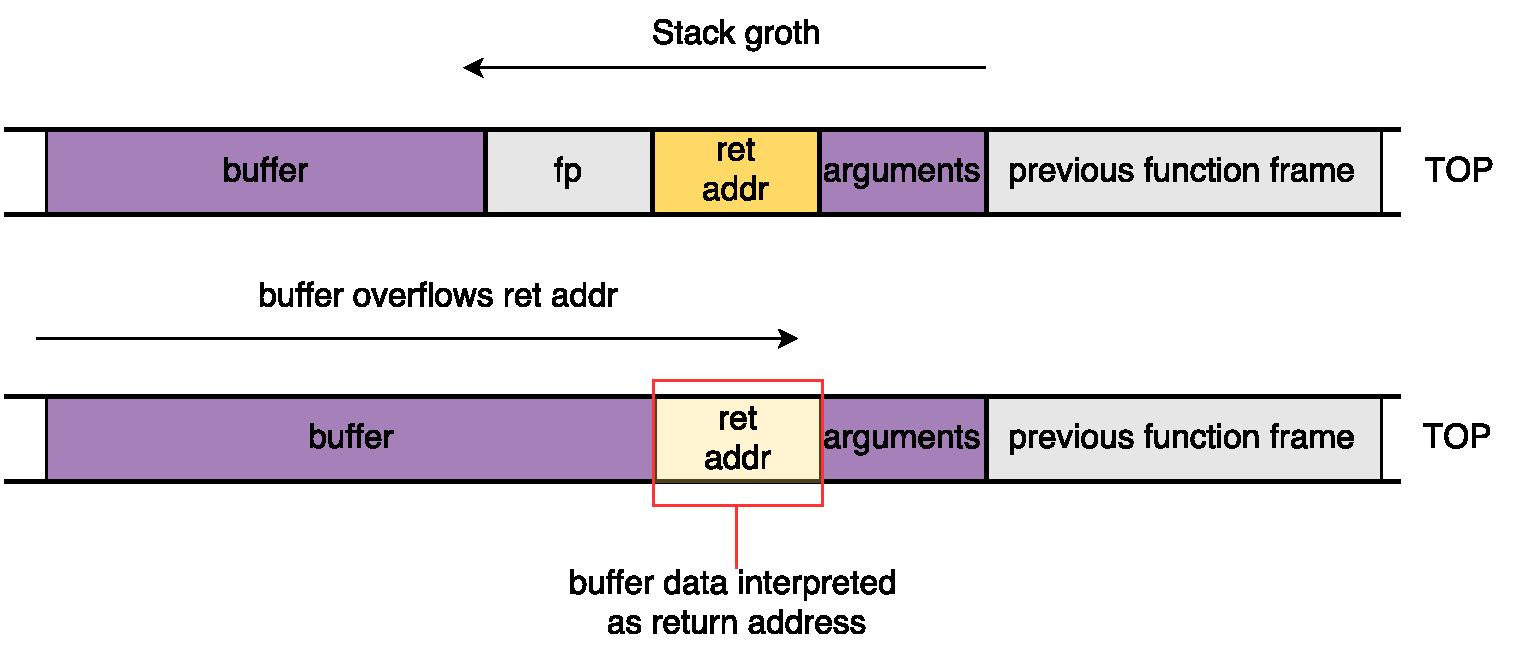
\includegraphics{figures/stackoverflow.pdf}
}
\end{center}
\end{figure}

\end{frame}

\begin{frame}
	\frametitle{Modify Pointer To Callback Function}
	Similar attack but operates also on heap ...
	\begin{itemize}
		\item Callback function pointer somewhere in heap
		\item Inject attack code by heap buffer overflow
		\item Change the function pointer to point to attack code
	\end{itemize}
\end{frame}

\begin{frame}
	\frametitle{Modify Pointer To Callback Function}
	\begin{figure}[!h]
\begin{center}
%\includegraphics[width=9cm]{figures/reader_states.jpg}
\scalebox{0.4}{%
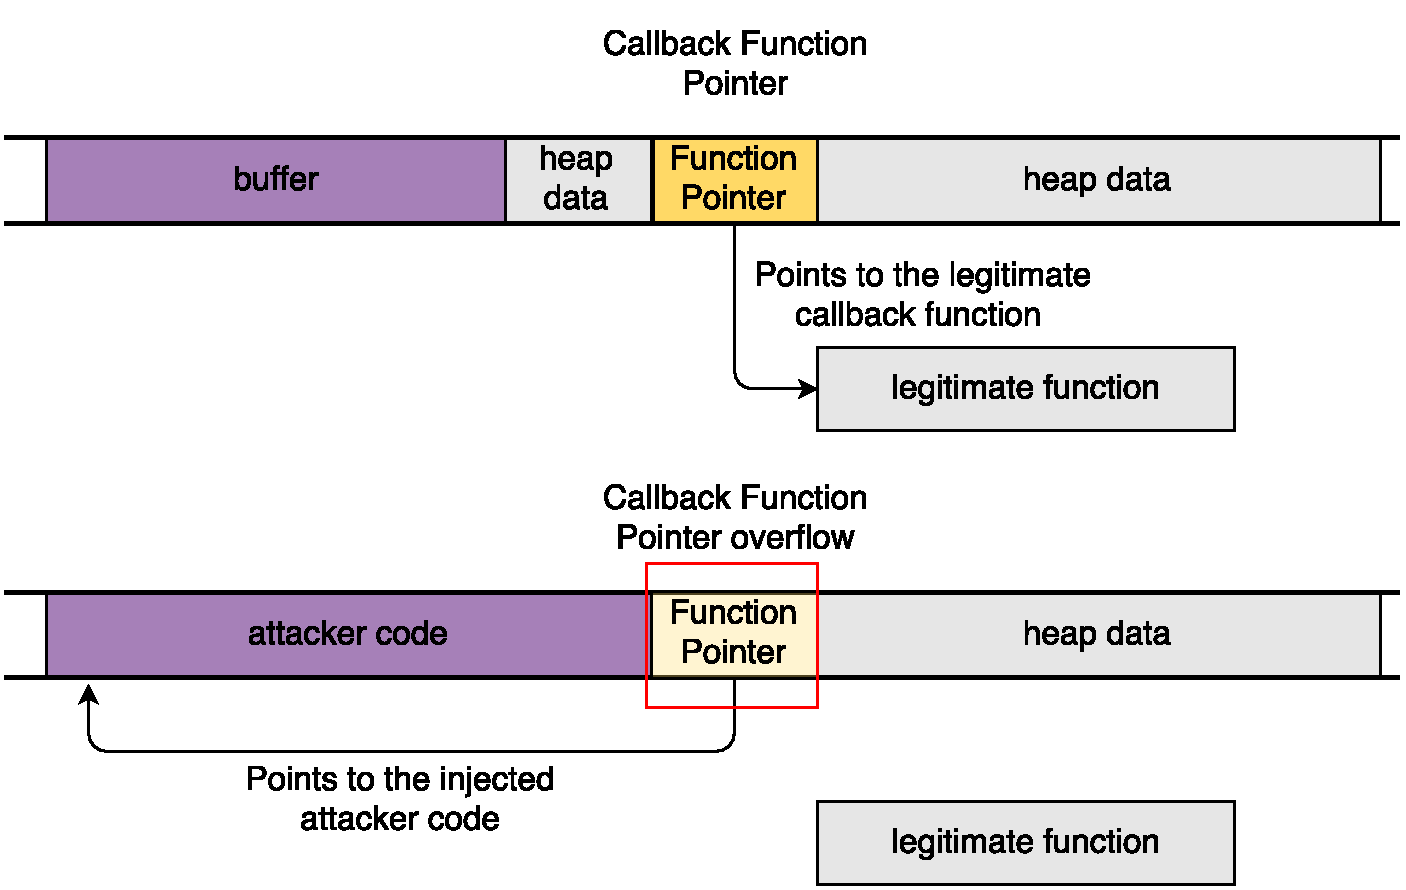
\includegraphics{figures/heap_callback_overflow.pdf}
}
\end{center}
\end{figure}

\end{frame}

\section{Rocket}
\begin{frame}
	\frametitle{Rocket}
	\begin{itemize}
		\item Open-Source, University of Berkeley
		\item Optimized instruction set for research topics (RISC-V)
		\item Developed with Chisel
		\item Currently tethered to ARM-Processor (boot-strapping)
		\item 64 bit, Single-Issue In-Order 5-stage pipeline
		\item 1.72 DMIPS/MHz
		 \item Clock rate \textgreater 1GHz
	\end{itemize}
\end{frame}

\begin{frame}
	\frametitle{Rocket Processor Structure}
	\begin{figure}[!h]
	\begin{center}
	%\includegraphics[width=9cm]{figures/reader_states.jpg}
		\scalebox{0.25}{%
		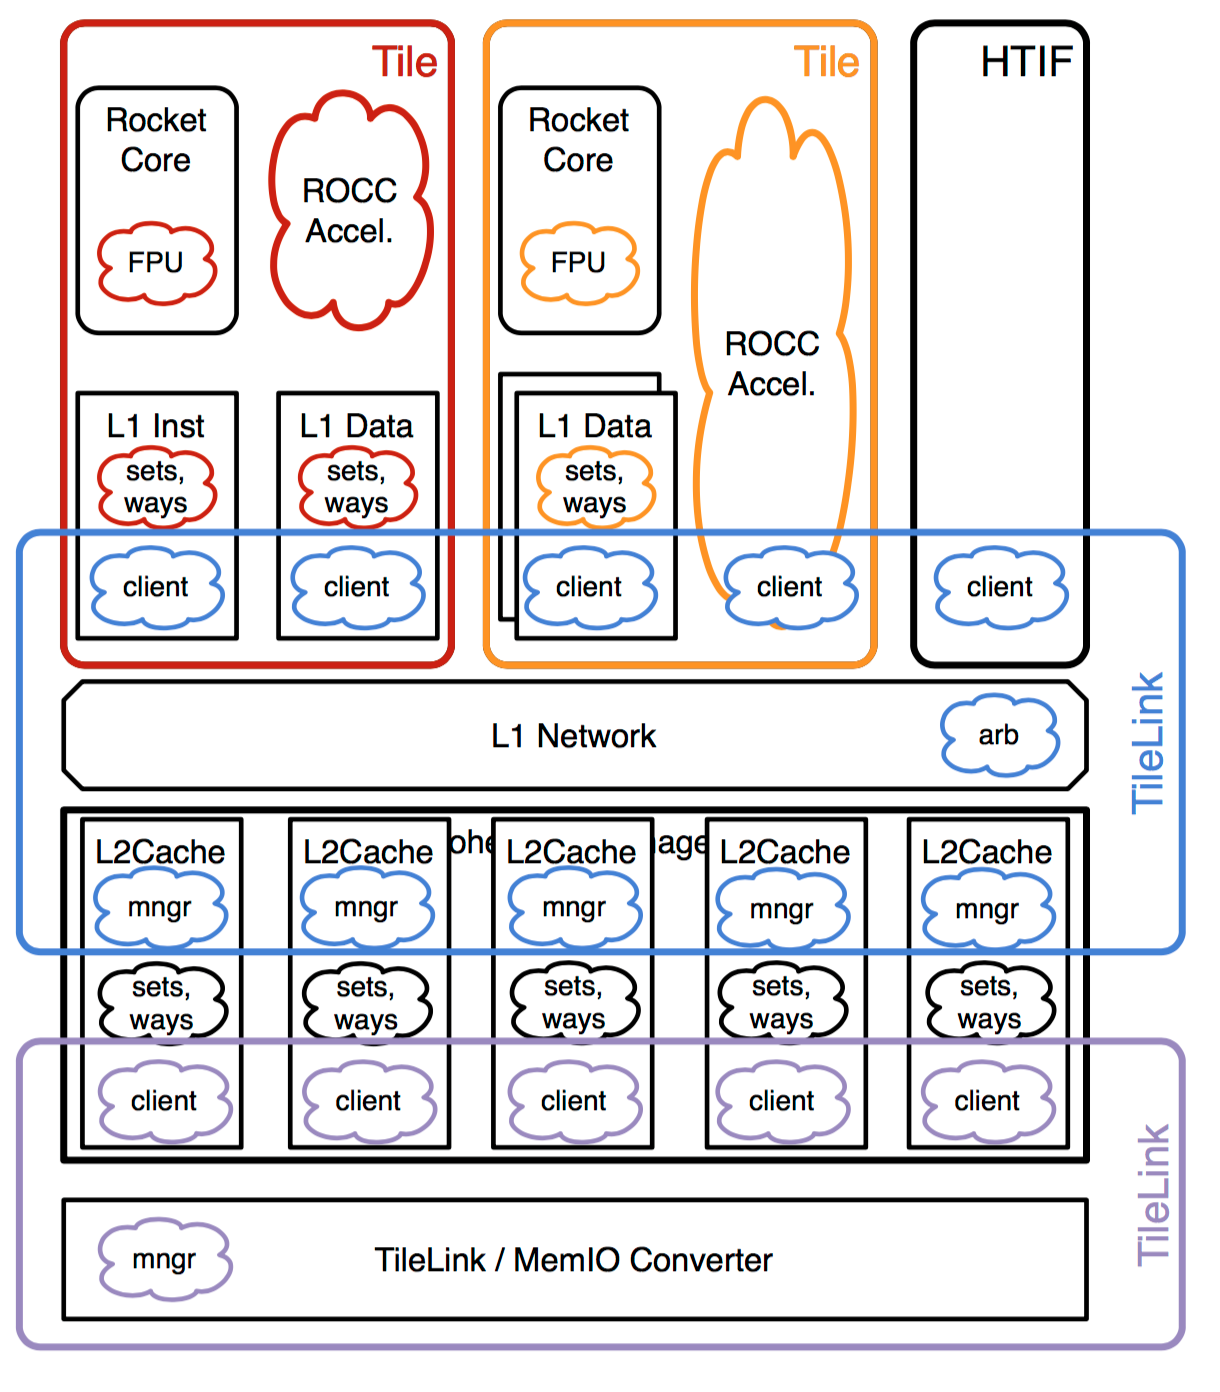
\includegraphics{figures/rocketoverview.png}
	}
	\end{center}
	\end{figure}
\end{frame}

\begin{frame}
	\frametitle{Chisel}
	Developed by University of Berkeley
	\begin{itemize}
		\item New high level hardware design language
		\item Based on Scala
		\item Full control over resulting RTL structures
		\item Powerful generator %(e.g add and remove modules per define)
		\item Outputs: Cycle accurate C++ emulator, Verilog
		\item Use Vectors, Maps, Objects within Scala
	\end{itemize}
\end{frame}

\begin{frame}
	\frametitle{RISC-V Toolchain}
	Several software tools for development
	\begin{itemize}
		\item Fully adapted GNU Toolchain
		\item RISC-V bare-metal compiler
		\item RISC-V Linux compiler
		\item Simulation with C++ emulator %(Waveform output included)
		\item FPGA-implementation using Verilog and Xilinx Vivado
	\end{itemize}
\end{frame}

\begin{frame}
	\frametitle{The lowRISC project}
		RISC-V at Cambridge 
		\begin{itemize}
		\item Goal to make a fully open SoC 
		\item Raspberry Pi for grown ups
		\item Community project to support hardware and application designers  
		\item Extend Rocket core with security features (tagged memory)
	\end{itemize}
\end{frame}

\section{Tagged Memory}
\begin{frame}
	\frametitle{Tagged Memory}
	Extension to Rocket by lowRISC team.
	\begin{itemize}
		\item Ability to tag every 64 bits in memory with one or more tag bits
		\item So far only framework (load and store tag)
		\item Area in DRAM reserved for tags
	\end{itemize}
	Changes to RISC-V
		\begin{itemize}
		\item Add L1 data cache support for tagged memory type
		\item TileLink size 512 to 544 bits to transfer data + tags
		\item Addition of Tag-Cache
	\end{itemize}
\end{frame}

\begin{frame}
	\frametitle{Tag-Cache}
\begin{figure}[!h]
	\begin{center}
	%\includegraphics[width=9cm]{figures/reader_states.jpg}
		\scalebox{0.2}{%
		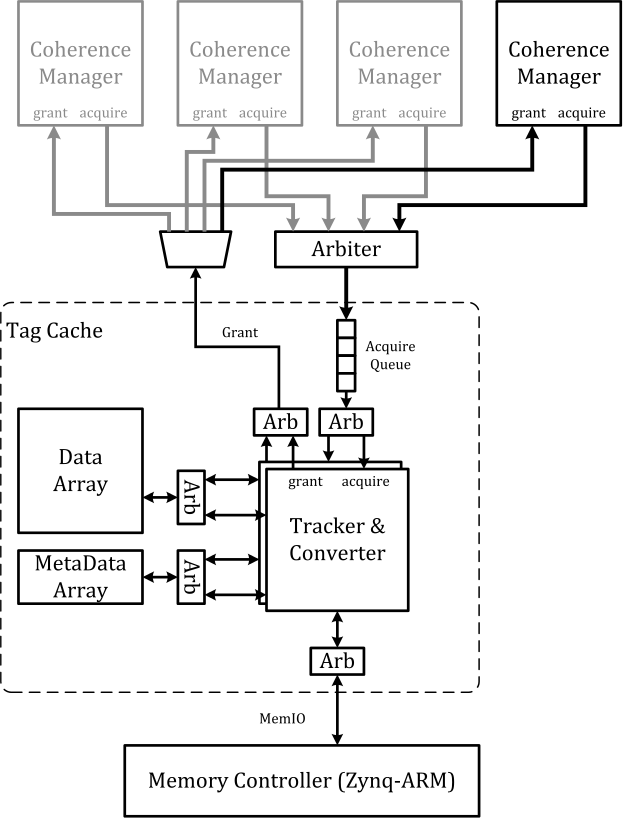
\includegraphics{figures/tag_cache.png}
	}
	\end{center}
	\end{figure}
\end{frame}

\section{Untethered Rocket}
\begin{frame}
	\frametitle{Current Rocket/ lowRISC}
	Tethered to ARM-Processing system (Zynq)
	\begin{itemize}
	\item HostIO: AXI Lite interface for input/output handled by ARM
	\item MemIO: AXI HP for DDR3 Memory access through ARM
	\item Boot strapping
	\item RISC-V Frontend Server handles console in/out
	\end{itemize}
\end{frame}

\begin{frame}
	\frametitle{Current Structure}
	\begin{figure}[!h]
		\begin{center}
	%\includegraphics[width=9cm]{figures/reader_states.jpg}
		\scalebox{0.38}{%
		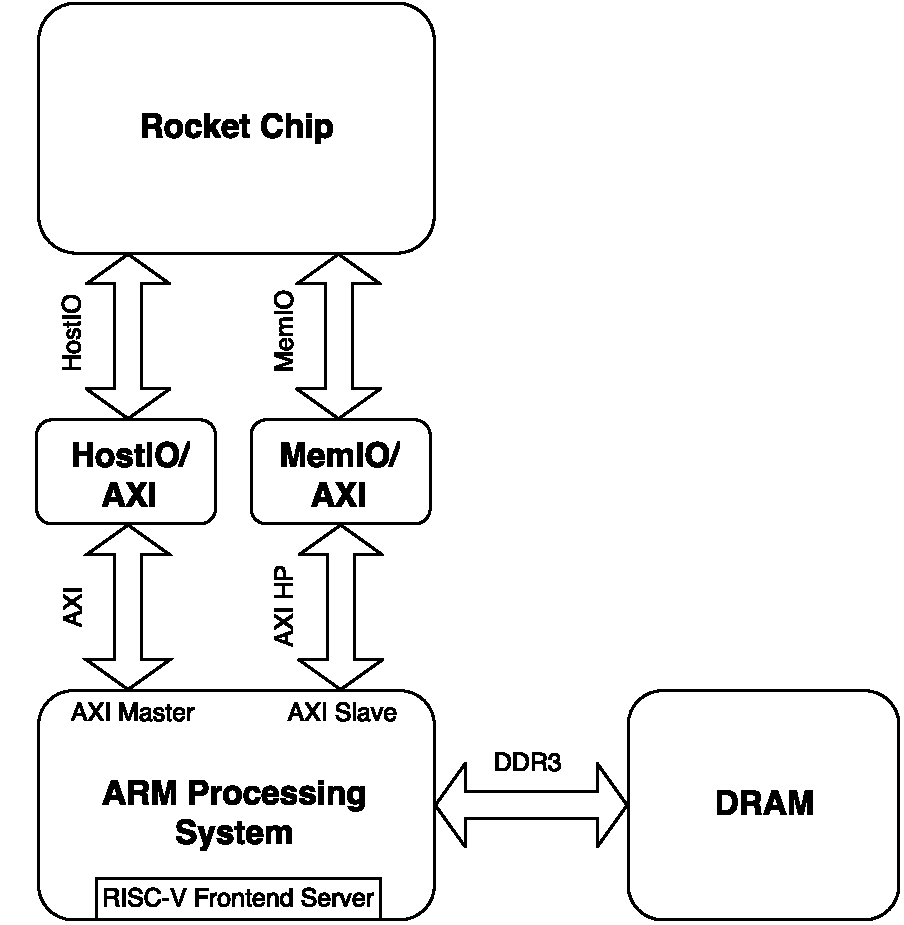
\includegraphics{figures/rocket_fpga_setup.pdf}
	}
	\end{center}
	\end{figure}
\end{frame}

\begin{frame}
	\frametitle{Changes for Untethering}
	lowRISC team implemented untethered version on Kintex-7 board
	\begin{itemize}
	\item MemIO exchanged with NASTI-Bus %(Berkley AXI-4 implementation)
	\item Memory mapped IO with NASTI-Lite
	\item Peripherals like UART and SPI for communication and debug
	\item Internal and external Bus width reduced to 128 bit %(4 bursts for one cache line)
	\item Tagged memory not ported yet
	\end{itemize}
\end{frame}

\begin{frame}
	\frametitle{Untethered Structure}
	\begin{figure}[!h]
	\begin{center}
	%\includegraphics[width=9cm]{figures/reader_states.jpg}
		\scalebox{0.32}{%
		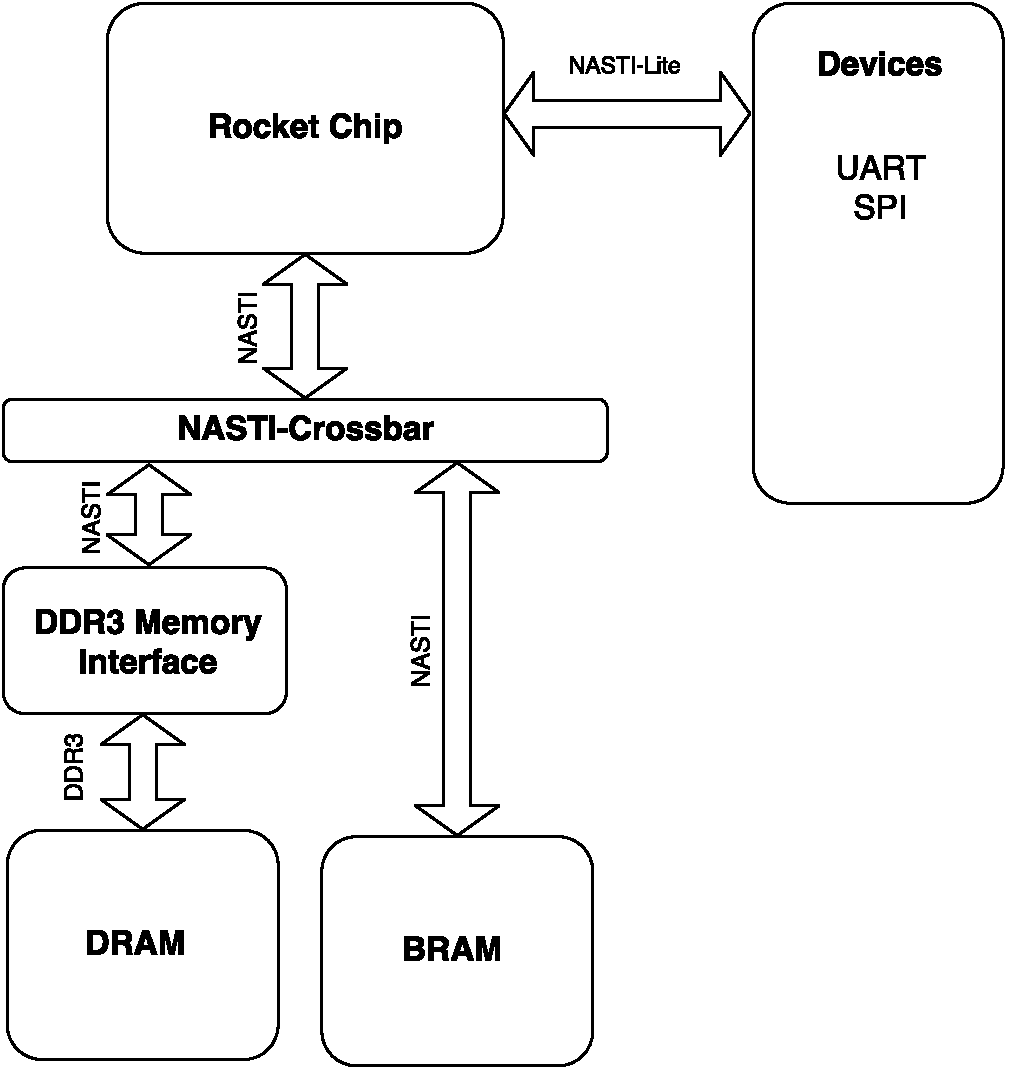
\includegraphics{figures/rocket_soc_setup.pdf}
	}
	\end{center}
	\end{figure}
\end{frame}

\section{Tag Security Policies}

\begin{frame}
	\frametitle{Tag Security Policies}
   Idea: Secure return address and function pointers from attackers
   \begin{itemize}
	   \item Only minor to no change to operating system (Linux context switch)
 	  \item Use of 2 tag bits per 64 bit data %(Bit 1: DATA/INVALID, Bit 2: RETURN)
 	  \item Implementation in untethered version
 	  \item Tag Control Unit that checks tags and causes traps/reset   
 	  \item Transparent for applications
   \end{itemize}
\end{frame}

\begin{frame}
	\frametitle{Return Address Protection}
	\begin{enumerate}
	\item Function Call: JAL stores return address to stack. Tags memory as RET
	\item Attacker overwrites return address. RET tag cleared.
	\item JAL-R tries to jump to address in RA register without tag (trap performed)
	\end{enumerate}
	\begin{figure}[!h]
		\begin{center}
	%\includegraphics[width=9cm]{figures/reader_states.jpg}
		\scalebox{0.35}{%
		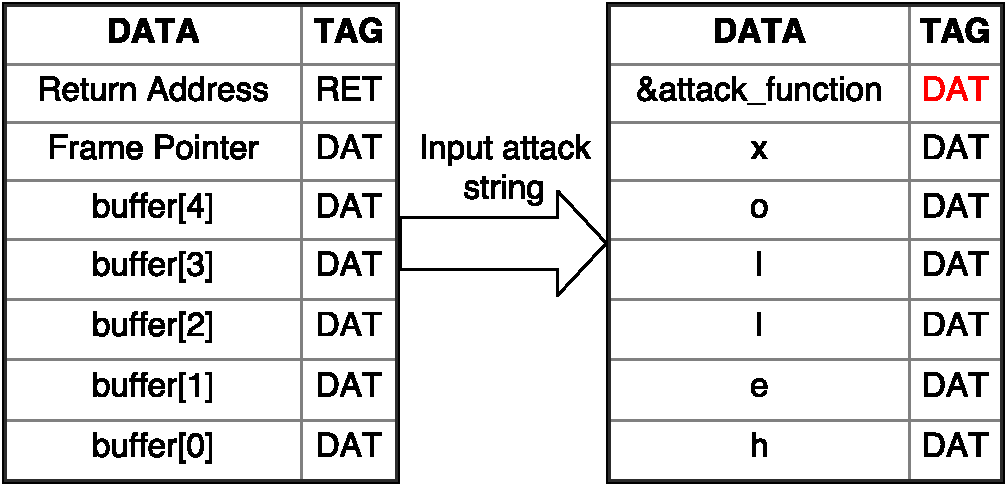
\includegraphics{figures/rat_address_tag.pdf}
	}
	\end{center}
	\end{figure}
\end{frame}

\begin{frame}
	\frametitle{Dynamic Taint Tracking}
	\begin{enumerate}
	\item Data and function pointers tagged as DATA
	\item Attacker injects code and overwrites function pointer. (IO input causes INV tag)
	\item JAL-R tries to jump to address with INV tag (trap performed)
	\end{enumerate}
	\begin{figure}[!h]
		\begin{center}
	%\includegraphics[width=9cm]{figures/reader_states.jpg}
		\scalebox{0.35}{%
		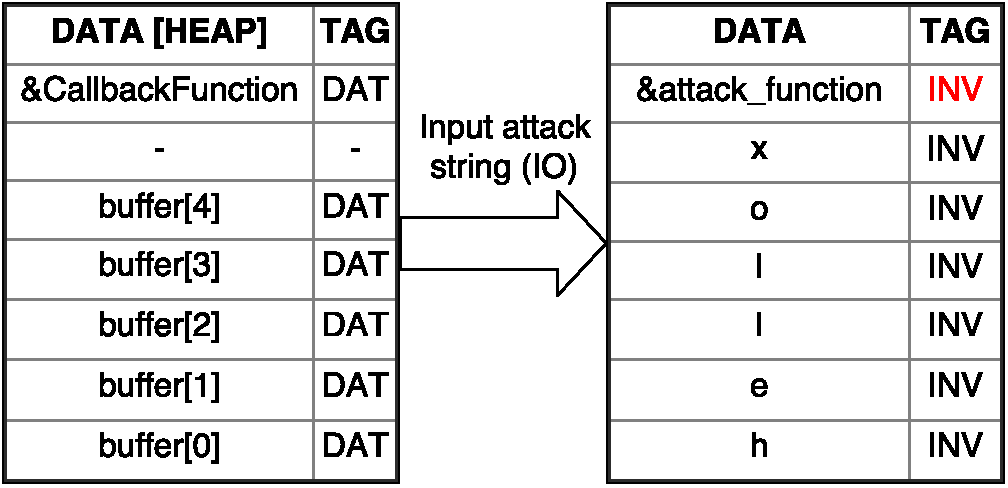
\includegraphics{figures/callback_fp_tag.pdf}
	}
	\end{center}
	\end{figure}
\end{frame}

\section{Project Time-line}

\begin{frame}
	\frametitle{Project Time-line}
   \begin{itemize}
   	  \item Preparation and lowRISC tutorial. 1.12.2015, 180h [Done]
	   \item Implementation of tagged memory. 31.01.2015, 150h
	   \item Tag security policies. 31.04.2015, 200h
		\item Documentation. 31.05.2015, 200h
   \end{itemize}
\end{frame}




%%%%%%%%%%%%%%%%%%%%%%%%%%%%%%%%%%%%%%%%%%%%%%%%%%%%%%%%%%%%%%%%%%%%%%%%%%%%
\end{document}
%%%%%%%%%%%%%%%%%%%%%%%%%%%%%%%%%%%%%%%%%%%%%%%%%%%%%%%%%%%%%%%%%%%%%%%%%%%%

%% EOF
